\documentclass[11pt,compress,t,notes=noshow, xcolor=table]{beamer}
\usepackage[]{graphicx}\usepackage[]{color}
% maxwidth is the original width if it is less than linewidth
% otherwise use linewidth (to make sure the graphics do not exceed the margin)
\makeatletter
\def\maxwidth{ %
  \ifdim\Gin@nat@width>\linewidth
    \linewidth
  \else
    \Gin@nat@width
  \fi
}
\makeatother

\definecolor{fgcolor}{rgb}{0.345, 0.345, 0.345}
\newcommand{\hlnum}[1]{\textcolor[rgb]{0.686,0.059,0.569}{#1}}%
\newcommand{\hlstr}[1]{\textcolor[rgb]{0.192,0.494,0.8}{#1}}%
\newcommand{\hlcom}[1]{\textcolor[rgb]{0.678,0.584,0.686}{\textit{#1}}}%
\newcommand{\hlopt}[1]{\textcolor[rgb]{0,0,0}{#1}}%
\newcommand{\hlstd}[1]{\textcolor[rgb]{0.345,0.345,0.345}{#1}}%
\newcommand{\hlkwa}[1]{\textcolor[rgb]{0.161,0.373,0.58}{\textbf{#1}}}%
\newcommand{\hlkwb}[1]{\textcolor[rgb]{0.69,0.353,0.396}{#1}}%
\newcommand{\hlkwc}[1]{\textcolor[rgb]{0.333,0.667,0.333}{#1}}%
\newcommand{\hlkwd}[1]{\textcolor[rgb]{0.737,0.353,0.396}{\textbf{#1}}}%
\let\hlipl\hlkwb

\usepackage{framed}
\makeatletter
\newenvironment{kframe}{%
 \def\at@end@of@kframe{}%
 \ifinner\ifhmode%
  \def\at@end@of@kframe{\end{minipage}}%
  \begin{minipage}{\columnwidth}%
 \fi\fi%
 \def\FrameCommand##1{\hskip\@totalleftmargin \hskip-\fboxsep
 \colorbox{shadecolor}{##1}\hskip-\fboxsep
     % There is no \\@totalrightmargin, so:
     \hskip-\linewidth \hskip-\@totalleftmargin \hskip\columnwidth}%
 \MakeFramed {\advance\hsize-\width
   \@totalleftmargin\z@ \linewidth\hsize
   \@setminipage}}%
 {\par\unskip\endMakeFramed%
 \at@end@of@kframe}
\makeatother

\definecolor{shadecolor}{rgb}{.97, .97, .97}
\definecolor{messagecolor}{rgb}{0, 0, 0}
\definecolor{warningcolor}{rgb}{1, 0, 1}
\definecolor{errorcolor}{rgb}{1, 0, 0}
\newenvironment{knitrout}{}{} % an empty environment to be redefined in TeX

\usepackage{alltt}
\newcommand{\SweaveOpts}[1]{}  % do not interfere with LaTeX
\newcommand{\SweaveInput}[1]{} % because they are not real TeX commands
\newcommand{\Sexpr}[1]{}       % will only be parsed by R



\usepackage[english]{babel}
\usepackage[utf8]{inputenc}

\usepackage{dsfont}
\usepackage{verbatim}
\usepackage{amsmath}
\usepackage{amsfonts}
\usepackage{bm}
\usepackage{csquotes}
\usepackage{multirow}
\usepackage{longtable}
\usepackage{booktabs}
\usepackage{enumerate}
\usepackage[absolute,overlay]{textpos}
\usepackage{psfrag}
\usepackage{algorithm}
\usepackage{algpseudocode}
\usepackage{eqnarray}
\usepackage{arydshln}
\usepackage{tabularx}
\usepackage{placeins}
\usepackage{tikz}
\usepackage{setspace}
\usepackage{colortbl}
\usepackage{mathtools}
\usepackage{wrapfig}
\usepackage{bm}
\usetikzlibrary{shapes,arrows,automata,positioning,calc,chains,trees, shadows}
\tikzset{
  %Define standard arrow tip
  >=stealth',
  %Define style for boxes
  punkt/.style={
    rectangle,
    rounded corners,
    draw=black, very thick,
    text width=6.5em,
    minimum height=2em,
    text centered},
  % Define arrow style
  pil/.style={
    ->,
    thick,
    shorten <=2pt,
    shorten >=2pt,}
}
\usepackage{subfig}


% Defines macros and environments
\input{../../style/common.tex}

%\usetheme{lmu-lecture}
\newcommand{\titlefigure}{figure_man/cost-curves-2.png}
\newcommand{\learninggoals}{
\item See the limitations of ROC curves
\item Understand the concepts of precision-recall and cost curves}
\usepackage{../../style/lmu-lecture}

\let\code=\texttt
\let\proglang=\textsf

\setkeys{Gin}{width=0.9\textwidth}

\title{Introduction to Machine Learning}
% \author{Bernd Bischl, Christoph Molnar, Daniel Schalk, Fabian Scheipl}
\institute{\href{https://compstat-lmu.github.io/lecture_i2ml/}{compstat-lmu.github.io/lecture\_i2ml}}
\date{}

\setbeamertemplate{frametitle}{\expandafter\uppercase\expandafter\insertframetitle}


\begin{document}


% This file loads R packages, configures knitr options and sets preamble.Rnw as parent file
% IF YOU MODIFY THIS, PLZ ALSO MODIFY setup.Rmd ACCORDINGLY...


% Defines macros and environments
\input{../../latex-math/basic-math.tex}
\input{../../latex-math/basic-ml.tex}
\input{../../latex-math/ml-automl.tex}
%! includes: basics-learners 

\lecturechapter{Evaluation: Beyond AUC}
\lecture{Introduction to Machine Learning}

% ------------------------------------------------------------------------------

% \begin{vbframe}{Beyond AUC}
% 
% Cost curves, precision-recall curves
% 
% \begin{itemize}
%   \item Confusion matrices give rise to a plethora of metrics.
%   \item Besides ROC curves and AUC, many alternative perspectives on evaluation 
%   can be derived from combining different ROC metrics.
%   \item For example, we can construct \textbf{precision-recall curves} which are 
%   often preferred in cases of strong class imbalance.
%   \item \textcolor{blue}{Fictional example, mini case study, ...?}
% \end{itemize} 
% 
% \centering 
% 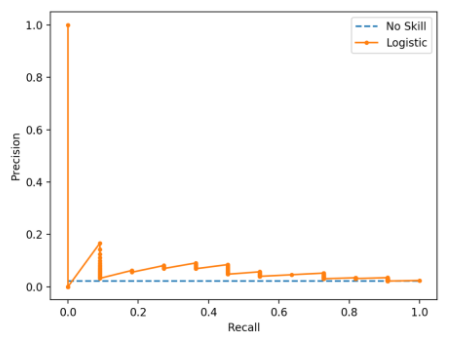
\includegraphics[width=0.3\textwidth]{figure_man/placeholder_precision_recall} 
% 
% \begin{itemize}
%   \item For practitioners it is vital to understand what should be 
%   evaluated exactly, and which measure is appropriate.  
% \end{itemize}
% 
% \end{vbframe}

% ------------------------------------------------------------------------------

\begin{vbframe}{Precision-Recall Curves}

%\textbf{Motivation}: ROC curves should mainly be used in binary classification 
%problems.

\begin{footnotesize}

When dealing with highly imbalanced data (i.e., $\nn \gg \np$), precision-recall 
(PR) curves may be more useful than ROC curves:
% of an algorithms performance.

\begin{itemize}
  \item Precision = $\frac{TP}{TP + FP}$, recall = TPR = $\frac{TP}{TP + FN}$ 
  (do not depend on TN).
  %\item Note that both measures are not dependent on true negatives.
  \item Figure (a): ROC curve shows that both algorithms perform well.
  \item Figure (b): PR curve shows that there is room for improvement (optimum 
  PR curve: top-right corner).
  \item The PR space reveals that algorithm 2 has an advantage over algorithm 1, 
  which is due to imbalanced classes.
\end{itemize}

\end{footnotesize}

\begin{figure}
  \centering
  \scalebox{0.8}{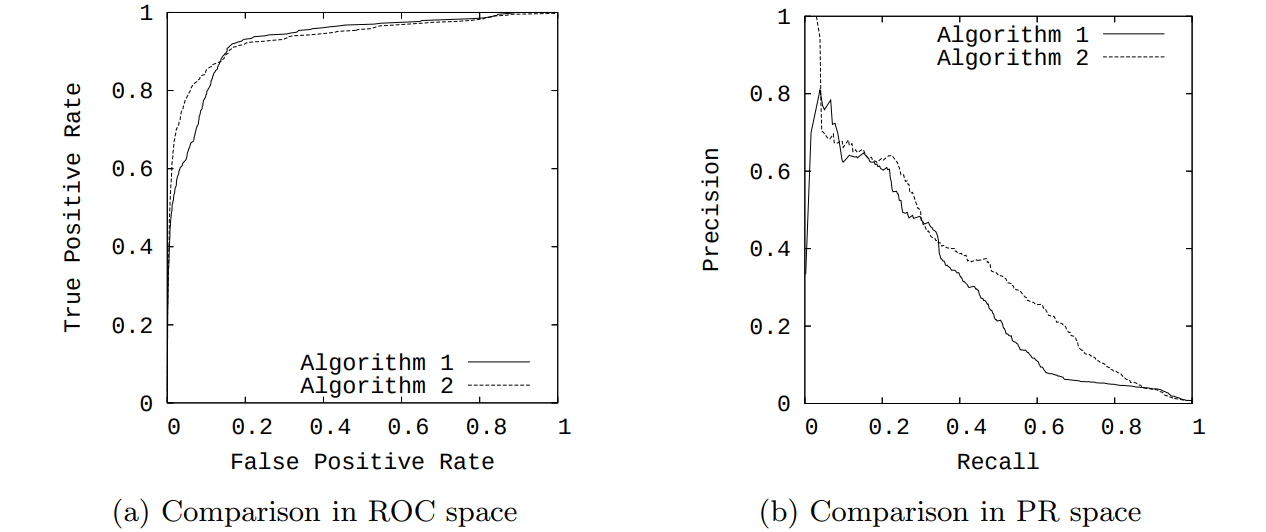
\includegraphics{figure_man/roc-pr.png}}
  \tiny
  \\Davis and Goadrich (2006): The Relationship Between Precision-Recall and 
  ROC Curves (\href{https://www.biostat.wisc.edu/~page/rocpr.pdf}
  {\underline{URL}}).
  % \tiny{\\ Credit: Jesse Davis and Mark Goadrich \\}
\end{figure}

% {\tiny{Davis and Goadrich (2006): The Relationship Between Precision-Recall and 
% ROC Curves (\href{https://www.biostat.wisc.edu/~page/rocpr.pdf}{\underline{URL}}). 
% \emph{\url{https://www.biostat.wisc.edu/~page/rocpr.pdf}}}\par}

% Source: http://people.cs.bris.ac.uk/~flach/ICML04tutorial/ROCtutorialPartI.pdf
%\tiny{Source for material: https://www.biostat.wisc.edu/~page/rocpr.pdf}
%\tiny{Source for material: https://towardsdatascience.com/what-metrics-should-we-use-on-imbalanced-data-set-precision-recall-roc-e2e79252aeba}
%\tiny{Source for material: https://machinelearningmastery.com/roc-curves-and-precision-recall-curves-for-classification-in-python/}
%\tiny{Source 6: http://binf.gmu.edu/mmasso/ROC101.pdf}
% Source: https://link.springer.com/content/pdf/10.1007/s10994-006-8199-5.pdf

\framebreak

\begin{itemize}
  \item The issue with ROC is the FPR in case of $\nn \gg \np$, which is often 
  very small as the TN are usually high. \newline
  $\Rightarrow$ A large change in FP yields a small change in the FPR.
  \item Precision: compares FP to TP (not TN) and does not suffer from this 
  issue. It captures the effect of the large $\nn$.
\end{itemize}

\begin{center}
  \includegraphics[width=0.8\textwidth]{figure_man/roc-confusion_matrix.png}
\end{center}

\framebreak

\begin{footnotesize}

\vspace{-0.2cm}
\begin{itemize}
  \item Figures in the top row concern imbalanced classes with $\pi = 0.003$, 
  those in the bottom row balanced ones with $\pi = 0.5$.
  \item Task and learners remain the same, only class distribution has changed.
  \item ROC curves (left) are similar, while the PR curve (right) changes 
  dramatically from imbalanced to balanced classes. 
  %\item Note that the superiority of classifiers in terms of performance can change with a skewed class distribution.
\end{itemize}

\end{footnotesize}

%replaced graph: (too small)
% \begin{figure}
%     \centering
%     \includegraphics[width=\textwidth]{figure_man/roc-pr-all.png}
%     \tiny{\\ Credit: Tom Fawcett \\}
% \end{figure}
% {\tiny{Tom Fawcett (2004): ROC Graphs: Notes and Practical Considerations for Researchers. \emph{\url{http://binf.gmu.edu/mmasso/ROC101.pdf}}}\par}

\begin{figure}
  \centering
  \scalebox{0.55}{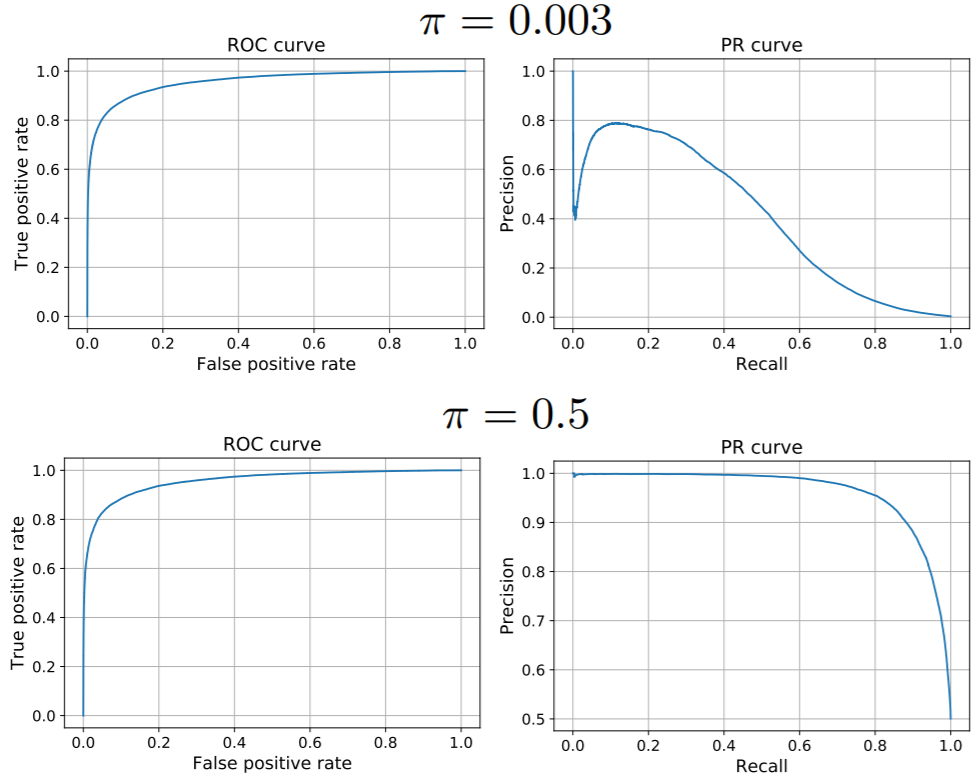
\includegraphics[width=\textwidth]
  {figure_man/roc-pr-imbalanced.png}}
  \tiny
  \\ Wissam Siblini et. al. (2004): Master your Metrics with Calibration 
  (\href{https://arxiv.org/pdf/1909.02827.pdf}{\underline{URL}}).
  % \tiny{\\ Wissam Siblini et. al. (2004): Master your Metrics with Calibration. 
  % \emph{\url{https://arxiv.org/pdf/1909.02827.pdf}}}\par
  % \tiny{\\ Credit: Wissam Siblini et. al. \\}
\end{figure}

% \vspace{-0.25cm}
% 
% {\tiny{Wissam Siblini et. al. (2004): Master your Metrics with Calibration. \emph{\url{https://arxiv.org/pdf/1909.02827.pdf}}}\par}

\framebreak

\textbf{Conclusion}: \\

\begin{itemize}
  \item ROC and PR curves for given algorithms contain the same points.
  %\item A curve that dominates in ROC space iff it dominates in PR space.
  \item Analogous to the convex hull in ROC space, there is a convex hull in PR 
  space (same points omitted as in convex hull in ROC space).
  \item An algorithm that optimizes the ROC-AUC is not guaranteed to optimize
  the PR-AUC.
  \begin{itemize}
    \item Use ROC curves when the numbers of samples in both classes are 
    roughly equal.
    \item Use PR curves when there is a moderate to large class
    imbalance and predicting positive instances is more relevant.
  \end{itemize}
\end{itemize}
\end{vbframe}

% ------------------------------------------------------------------------------

\begin{vbframe}{Cost curves}

\begin{itemize}
  \item \textbf{Cost curves} directly plot the relative costs / 
  misclassification error to determine the best classifier (ROC isometrics allow 
  this only indirectly).
  %\item Determining the superiority of a classifier can be difficult using the ROC isometrics.
  \item Cost curves incorporate similar information as ROC curves but are 
  easier, especially in case of different misclassification costs or class 
  distributions. %, or more generally the skew are known.
\end{itemize}

%\tiny{Source for material: Evaluating Learning Algorithms Chapter 4.4.3}
\vspace{-0.1cm}

\begin{minipage}{0.5\textwidth}
  \small
  \raggedright
  \textbf{Example:} Classifier $f_2$ dominates $f_1$ until both ROC curves 
  cross. Then, $f_1$ dominates $f_2$. \\
  \textbf{BUT:} It is hard to tell for which threshold, costs, or class 
  distributions $f_2$ works better than $f_1$. \\
  $\Rightarrow$ Cost curves provide this kind of information.
\end{minipage}
\begin{minipage}{0.49\textwidth}
  \begin{figure}
    \centering
    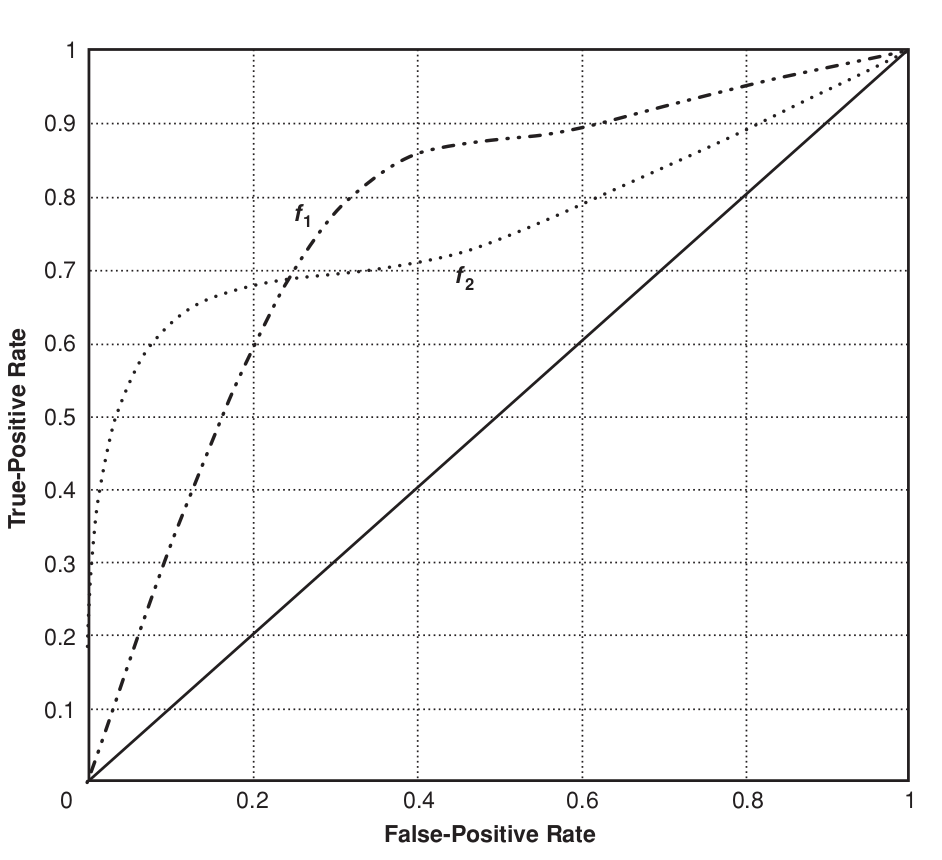
\includegraphics[width=0.8\textwidth]{figure_man/cost-curves-1.png}
    \tiny
    \\Nathalie Japkowicz (2004): Evaluating Learning Algorithms : A 
    Classification Perspective. (p. 125)
  \end{figure}
\end{minipage}

%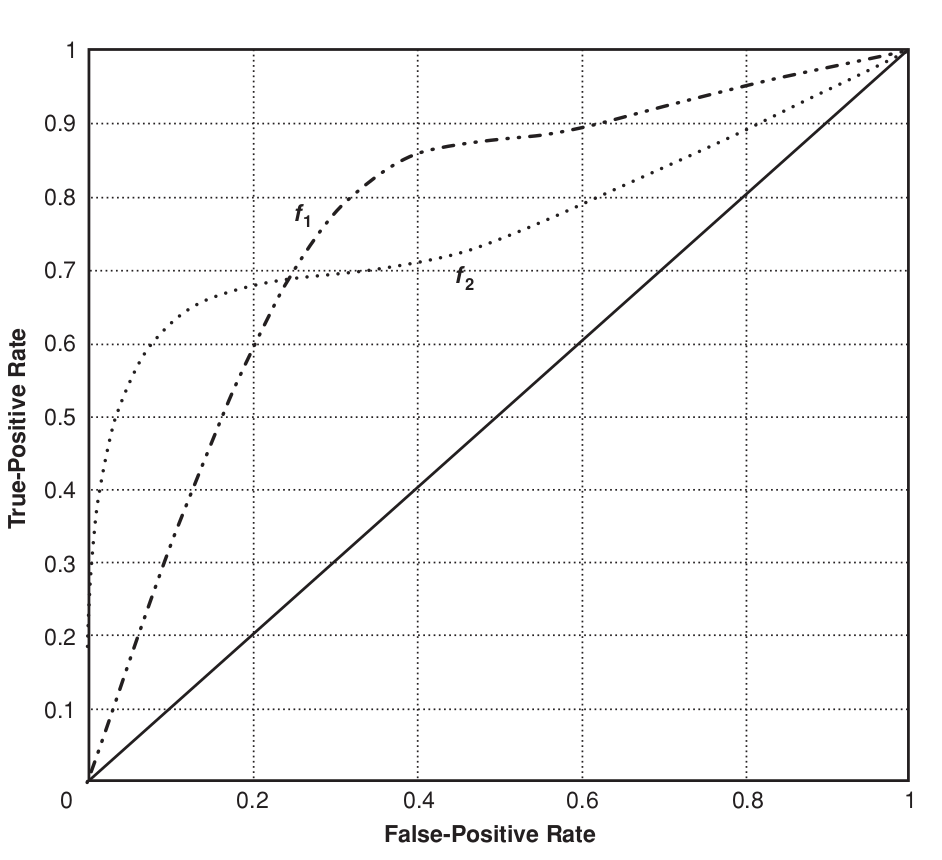
\includegraphics[width=\textwidth]{figure_man/cost-curves-1.png}
% \end{minipage}
% \vspace{1.5 cm}
% {\tiny{Nathalie Japkowicz (2004): Evaluating Learning Algorithms : A Classification Perspective. (p. 125)}}

\end{vbframe}

% ------------------------------------------------------------------------------

\begin{vbframe}{Cost curves}

\begin{footnotesize}

\begin{itemize}
  \item Simplifying assumption: equal misclassification costs, i.e., 
  $cost_{FN} = cost_{FP}$.
  \item Misclassification cost (or misclassification error in the case of 
  $cost_{FN} = cost_{FP}$) is plotted as a function of the proportion of 
  positive instances, $\rp$.
  \item Cost curves are point–line duals of ROC curves, i.e., a single 
  classifier is represented by a point in the ROC space and by a line in the 
  cost space.
\end{itemize}

\end{footnotesize}

\begin{figure}
  \centering
  \scalebox{0.8}{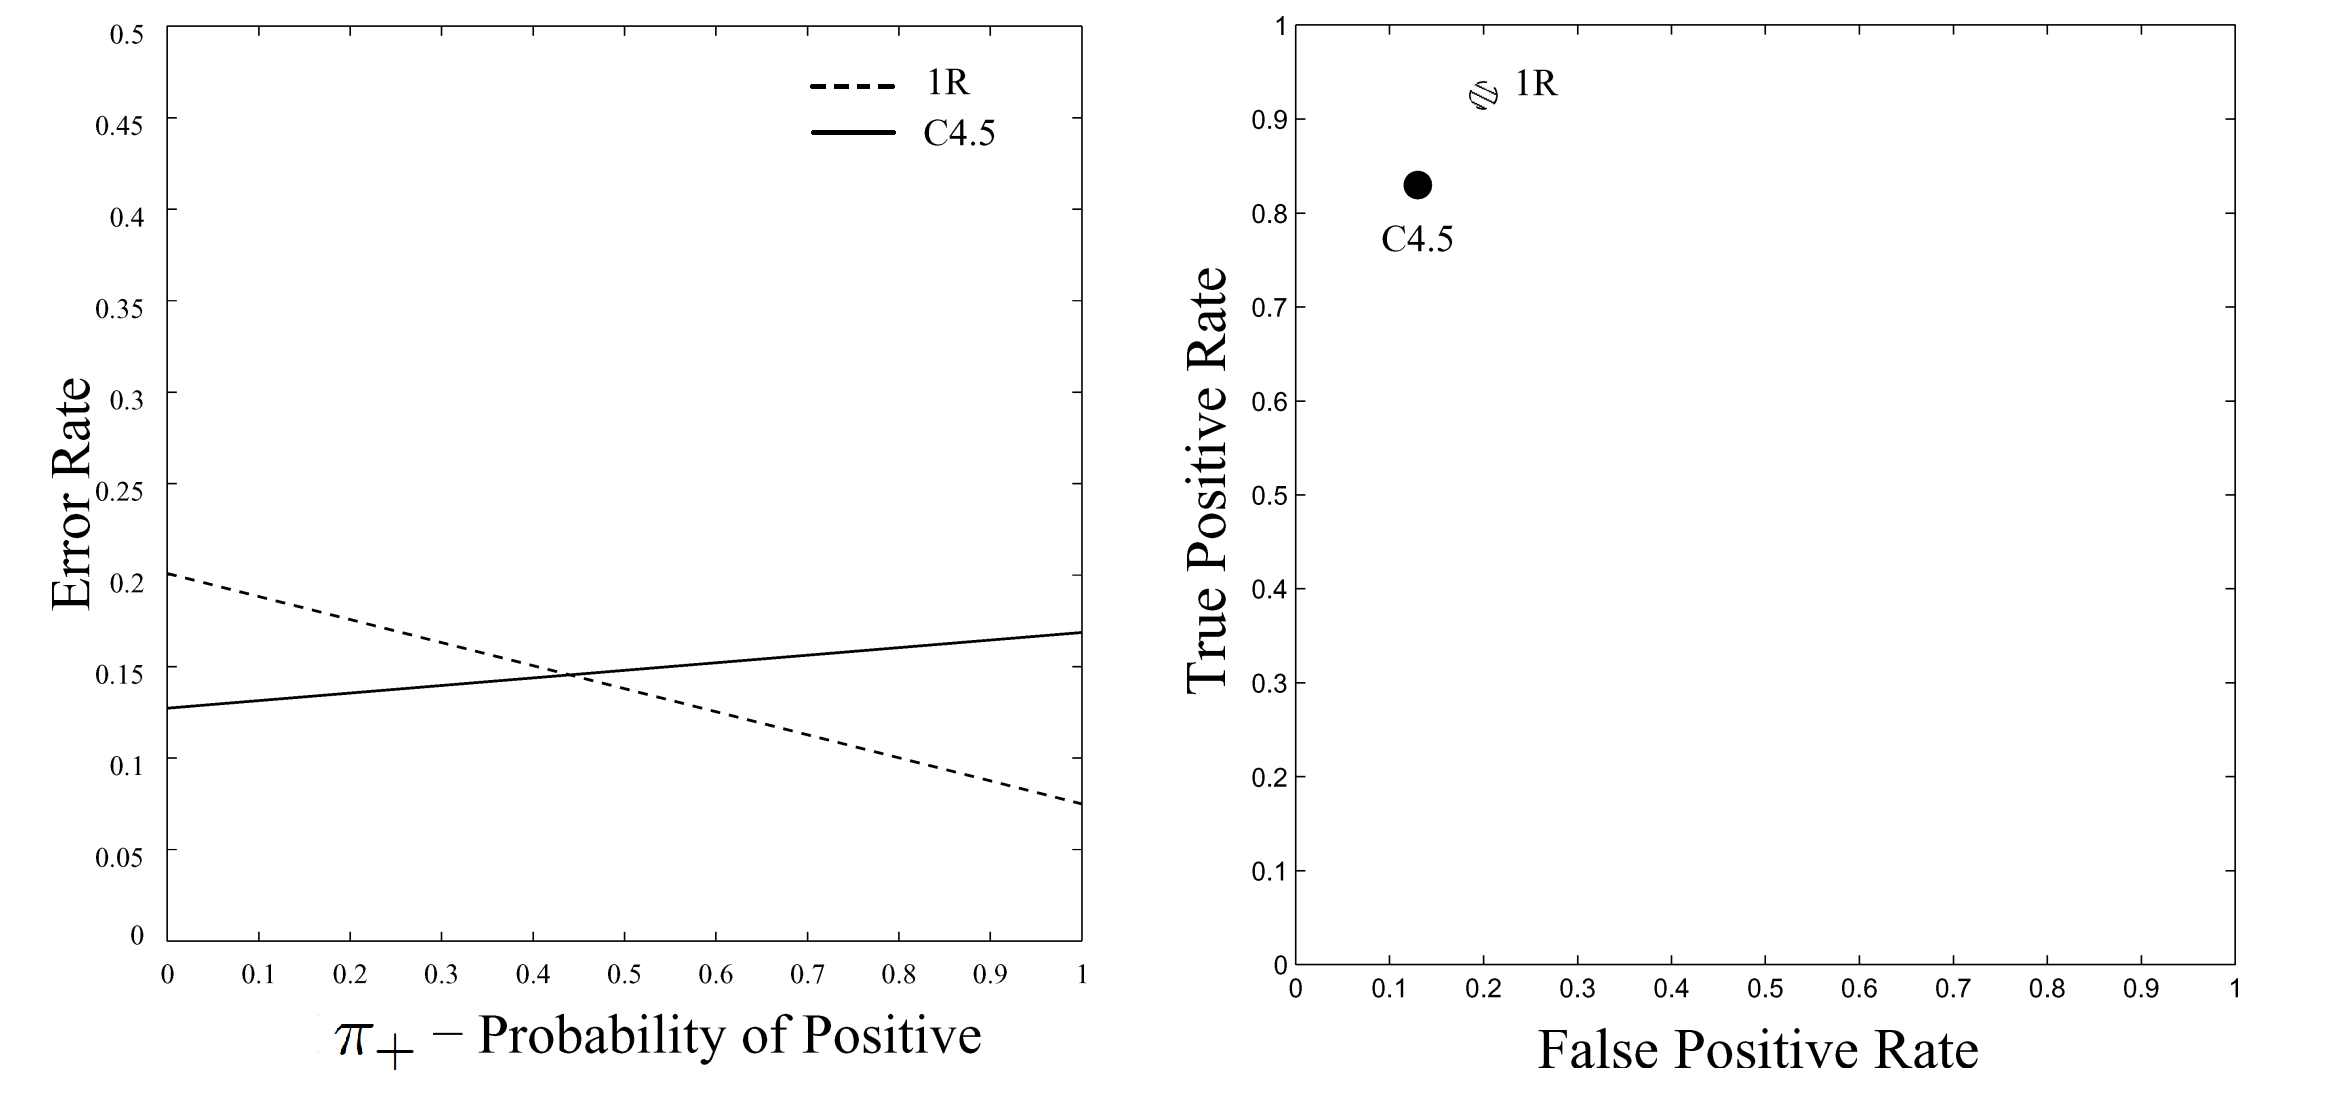
\includegraphics[width=\textwidth]
  {figure_man/cost-curves-0.png}}
  \tiny
  \\Chris Drummond and Robert C. Holte (2006): Cost curves: An improved
  method for visualizing classifier performance. \\Machine Learning, 65, 95-130 
  (\href{https://www.semanticscholar.org/paper/Cost-curves\%3A-An-improved-method-for  -visualizing-Drummond-Holte/71708ce984e0896e7383435913547e770572410e}
  {\underline{URL}}).
  % \tiny{\\ Credit: Chris Drummond and Robert C. Holte  \\}
\end{figure}

% {\tiny{Chris Drummond and Robert C. Holte (2006): Cost curves: An improved 
% method for visualizing classifier performance. Machine Learning, 65, 95-130. 
% \emph{\url{https://www.semanticscholar.org/paper/Cost-curves\%3A-An-improved-method-for-visualizing-Drummond-Holte/71708ce984e0896e7383435913547e770572410e}}}\par}

\end{vbframe}

% ------------------------------------------------------------------------------

\begin{vbframe}{Cost curves}

% \begin{itemize}
  %\item The convex hull of the ROC space is the lower envelope created of all classifier lines in the cost space.
  %\item The misclassification error is plotted as a function of the probability of an observation being from the positive class.
%   \item Functional form of the cost curve of a classifier:
%   $error = (FNR - FPR) \cdot \rp + FPR$ %, \;\;\;$ (Note: $P(+) = \rp$)
% \end{itemize}

Functional form of the cost curve of a classifier: 
$error = (FNR - FPR) \cdot \rp + FPR$.

\begin{center}
  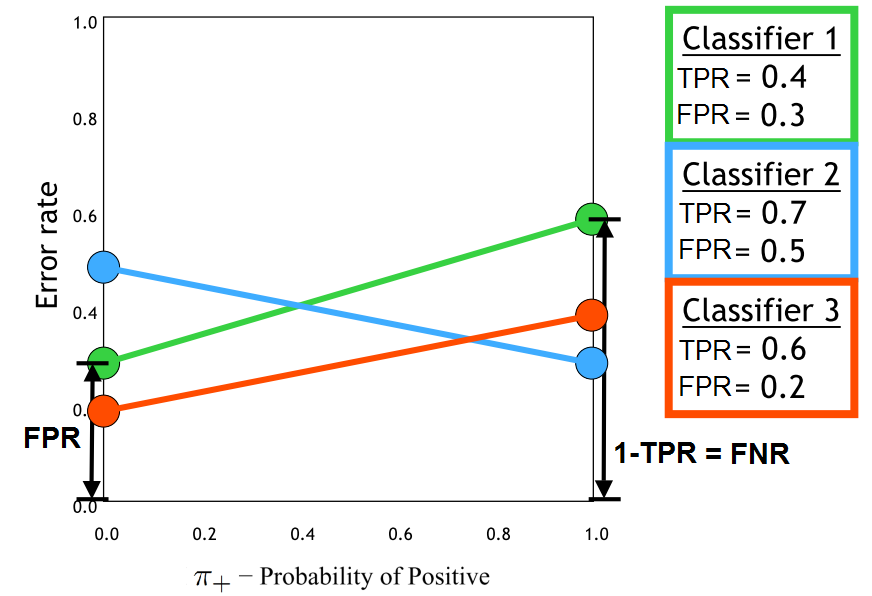
\includegraphics[width=0.85\textwidth]{figure_man/cost-curves-3.png}
\end{center}

\end{vbframe}

% ------------------------------------------------------------------------------

\begin{vbframe}{Cost curves}

\begin{footnotesize}

\begin{itemize}
  \item Horizontal dashed line: worst classifier, i.e. 100\% error rate for all 
  $\rp$; x-axis as perfect classifier.
  \item Dashed diagonal lines: trivial classifiers, i.e., ascending diagonal 
  always predicts negative instances and vice versa.
  \item Descending/ascending straight lines:
  two families of classifiers $A$ and $B$ (represented by points in their 
  respective ROC curves).
\end{itemize}

\end{footnotesize}

\begin{center}
  \scalebox{0.65}{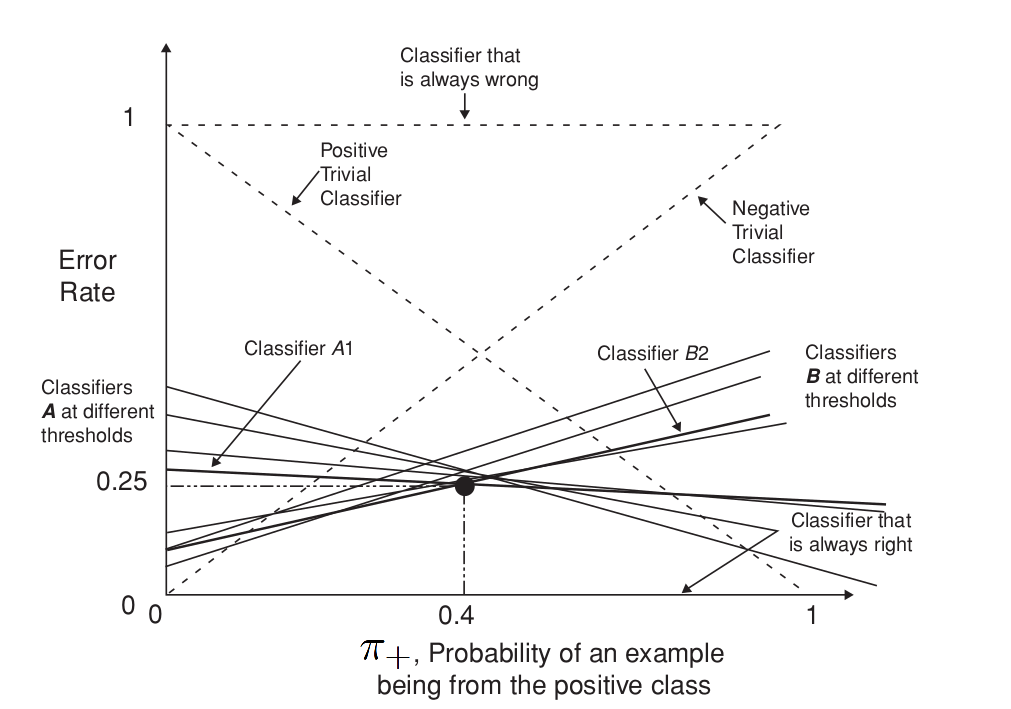
\includegraphics{figure_man/cost-curves-2.png}}
  \tiny{\\ Credit: Nathalie Japkowicz  \\}
\end{center}

\end{vbframe}

% ------------------------------------------------------------------------------

% \begin{vbframe}{Cost curves}
%
% \textbf{Example:} In position (0.4, 0.25) B classifier loses its
% performance to one of the A classifiers (point where ROC curves cross). But
% there is no practical information about when classifier A should be used
% over B. In contrast the cost graph tells us that for $0.26 \leq \rp < 0.4$
% classifier B is preferred and for $0.4 \leq \rp < 0.48$ classifier A1 is
% preferred.
%
% \begin{center}
% 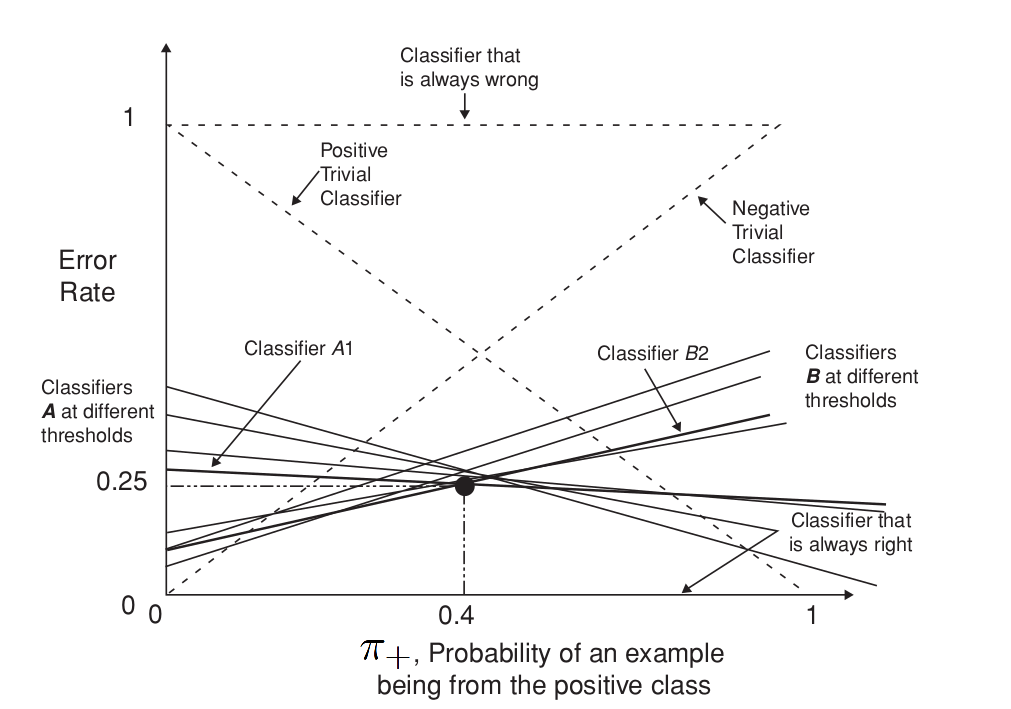
\includegraphics[width=0.5\textwidth]{figure_man/cost-curves-2.png}
% \end{center}
%
% \end{vbframe}

% ------------------------------------------------------------------------------

\begin{vbframe}{ROC curves vs. cost curves}

\begin{itemize}
  \item In some cases, cost curves provide more practical relevant information
  than ROC curves.
  \item ROC curves can tell us that, sometimes, classifier A is superior to B, 
  but we cannot really tell in which settings.
  \item Here, we assumed that the classes had similar classification costs.
  \item However, there is an extension to the cost curve concept which allows 
  for different costs in each class ($\rightarrow$ simple modification where the 
  identity of the axes is changed).
  %\item Then, the y-axis represents the normalized expected cost (NEC) or relative expected misclassification cost.
  \end{itemize}

\end{vbframe}

% ------------------------------------------------------------------------------

% \begin{vbframe}{ROC curves vs. cost curves}
% The general form is as follows:
%
% \vspace{-0.5cm}
% \begin{center}
% \begin{equation*}
% NEC = \text{FNR} \cdot P_C[+] + \text{FPR} \cdot (1 - P_C[+]),
% \end{equation*}
% \end{center}
%
% \begin{itemize}
% \item FNR/FPR are false-negative rate and false-positive rate respectively and
% $P_C[+]$, the probability cost function (modified version of $P[+]$ that takes costs into
% consideration).
%
% \vspace{-0.5cm}
% \begin{center}
% \begin{equation*}
% P_C[+] = \frac{P[+] \cdot C[+|-]}{P[+] \cdot C[+|-] + P[-] \cdot C[-|+]},
% \end{equation*}
% \end{center}
%
% \item $C[+|-]$ and $C[-|+]$ represent the cost of predicting a positive when the
% instance is actually negative and vice versa and $P[-]$ as the probability of
% being in the negative class.
% \end{itemize}
% \end{vbframe}

% ------------------------------------------------------------------------------

\endlecture
\end{document}
